\documentclass[addpoints,12pt]{exam}
%\documentclass[12pt]{article}
\usepackage[letterpaper, margin=0.75in]{geometry}
\usepackage{graphicx}
\usepackage{enumitem}
\usepackage{booktabs}
\usepackage{tabularx}
\usepackage{color}
\usepackage{wrapfig}

\begin{document}
\footer{}{Page \thepage\ of \numpages}{}

\begin{flushright}
\makebox[0.5\textwidth]{\large Name:\enspace\hrulefill}
\vspace{0.2in}

\end{flushright}

\begin{center}
\includegraphics[width=10cm]{../images/logo.png}
\end{center}

\begin{center}
\noindent{\LARGE Conceptual Physics \\ First Partial Test\\ March 30, 2018 \\}
\end{center}

\vspace{0.5in}

\begin{large}
You are free to use all notes on your two-sided cheat sheet. There are extra blank sheets at the end, which can be used for calculations, and if you require more please ask and be sure to include them when you hand back the test. Please be sure to include all your work and calculations.

Some useful geometric quantities for this test may include:
\begin{eqnarray}
\textrm{Area of a Circle} &=& \pi\times(\textrm{radius})^2 \nonumber \\
\textrm{Area of a Triangle} &=& \frac{1}{2}\textrm{base}\times\textrm{height}  \nonumber \\
\textrm{Area of a Rectangle} &=& \texttt{base}\times\textrm{height}\nonumber
\end{eqnarray}

There are \numquestions ~ problems for a total of \numpoints ~ points. (One of the questions is a bonus though.)
\end{large}
\vspace{0.2in}


 
\clearpage

\begin{flushright}
Score: \hspace{0.2in} / \numpoints ~ points
\end{flushright}

\begin{questions}
\question \textbf{Jupiter's Moons:} Jupiter is the largest planet in our solar system, and has 53 named moons (although NASA scientists think it has a total of 69 moons). The largest one is called \textit{Ganymede}. Most orbits are not perfectly circular, and are in fact shaped like ellipses. In the diagram below, images (I), (II), (III) and (IV) show snapshots in time of Jupiter and its largest moon in orbit around it. Use these images to answer the following questions. \textbf{For each question, please also \textit{explain your answer}.}

\begin{center}\input{../images/jupiter.pdf_tex}\end{center}

\begin{parts}
\part[2] At which instant (I, II, III, IV) is the \textit{gravitational force} between Jupiter and Ganymede the \textit{greatest}? \textbf{Why?}
	\begin{TheSolution}
		\textbf{III.} The gravitational force is greatest when the two are closest together.
	\end{TheSolution}
\part[2] At which instant (I, II, III, IV) is the \textit{gravitational potential energy} between Jupiter and Ganymede the \textit{greatest}? \textbf{Why?}
	\begin{TheSolution}
		\textbf{I.} Gravity is an attractive force, and so the gravitational potential energy is greatest when the two are furthest apart.
	\end{TheSolution}
\part[2] Assume energy is conserved in the Jupiter/Ganymede system. At which instant (if any) is the Ganymede's \textit{speed} the \textit{greatest}? \textbf{Why?}
	\begin{TheSolution}
		\textbf{III.} If energy is conserved, then the sum of the kinetic and gravitational potential energies is a constant. Thus when the gravitational potential energy is the smallest, the kinetic energy is the greatest. This occurs at point III, when the two are closest together. If the kinetic energy is very large, then the speed of the moon is the greatest (since as speed increases, kinetic energy also increases).
	\end{TheSolution}
\end{parts}

\begin{minipage}{\linewidth}
\begin{wrapfigure}{R}{0.3\textwidth}
	\vspace{-20pt}
	\begin{center}\includegraphics[width=0.3\textwidth]{../images/freediving.jpg}\end{center}
	\vspace{-20pt}
\end{wrapfigure}
\question \textbf{Free Diving:} In free diving, athletes hold there breath and descend as far as possible (\textit{without} using air tanks, like in scuba diving). Often, they use a guide rope to descend and ascend back to the surface, as well as weights to pull them down and fins to rise. The image on the right shows a freediver with a guide rope.

The graph below shows the \textit{velocity as a function of time} for an athlete as she descends (from 0 to 31 seconds), pauses for a moment (from 31 to 35 seconds), and then ascends back to the surface (from 35 to 51 seconds).

\begin{center}
\includegraphics[width=0.9\textwidth]{../images/test1V2_freeDiving.png}
\end{center}

\begin{parts}
	\part[2] When during her dive does the athlete experience \textit{zero acceleration}? Provide all time interval(s). If she never experiences zero acceleration, provide an explanation.
		\begin{TheSolution}
			Acceleration is zero when velocity is not changing (the velocity versus time graph is flat). This happens:
			\begin{enumerate}
				\item between t=1s and t=30s
				\item between t=31s and t=35s
				\item between t=36s and t=50s
			\end{enumerate}
		\end{TheSolution}
	\part[2] When during her dive does the athlete experience \textit{negative acceleration} (accelerating \textit{down})? Provide all time interval(s). If she never experiences negative acceleration, provide an explanation.
		\begin{TheSolution}
			Negative acceleration occurs when the graph is pointing down. This happens at:
			\begin{enumerate}
				\item t=0s and t=1s
				\item t=50s and t=51s
			\end{enumerate}
		\end{TheSolution}
	\part[2] How deep did the athlete descend?
		\begin{TheSolution}
			\textbf{180 m} The area under a velocity vs. time graph gives displacement. We could therefore use the area under the first or second part of the graph, since one will be negative (as she descends) and the other will be positive (as she ascends).
			\begin{eqnarray}
				area = base\times height = -6 m/s \times 30s = -180m
				area = base\times height = 12 m/s \times (50s-35s) = 180m
			\end{eqnarray}
		\end{TheSolution}
\end{parts}
\end{minipage}

\clearpage

\question \textbf{Smashing Protons:} In particle accelerators, subatomic particles (such as protons) are accelerated to very large speeds and then collide with one another. The resulting high-energy collisions produce other particles, which researchers use to test models of particle physics. However, not all particles in the accelerators collide (since they are very hard to align): Often their trajectories are off and they simply deflect. The diagram bellow illustrates a situation like this. Two protons are accelerated towards one another, but instead of colliding they deflect each other. The dashed lines illustrate their respective paths, and their simultaneous positions at different points in time are labeled as (I), (II), (III), (IV) and (V). Please use these labels to answer the following questions. \textbf{For each question, please also \textit{explain your answer}.}
	
	\noindent\begin{center}\input{../images/smashing_protons.pdf_tex}\end{center}
	
	\begin{parts}
	\part[2] At what point(s) in time (I, II, III, IV, V) do the protons feel an electrical force? \textbf{Why?}
		\begin{TheSolution}
			All points (I, II, II, IV, V). The electromagnetic force extends throughout all space (it has infinite range) and so at all points in time the two feel a repulsion.
		\end{TheSolution}
	\part[2] At what point(s) in time (I, II, III, IV, V) do the protons experience the \textit{greatest electric force}? \textbf{Why?}
		\begin{TheSolution}
			\textbf{III.} The force is greatest when the two are closest together.
		\end{TheSolution}
	\part[2] At what point(s) in time (if any) does the proton/proton system have the \textit{greatest electric potential energy}?\textbf{ Why?}
		\begin{TheSolution}
			\textbf{III.} The two experience a repulsive force, and so their potential energy is greatest when the are closest together.
		\end{TheSolution}
	\end{parts}

\clearpage

\bonusquestion In \textit{nuclear fusion}, atomic nuclei come together, forming larger nuclei. The process releases nuclear potential energy, and occurs naturally in stars. In the \textit{triple-alpha process} three helium nuclei come together, forming carbon (by forming an intermediate beryllium nucleus). The figure bellow illustrates this process:

\begin{center}
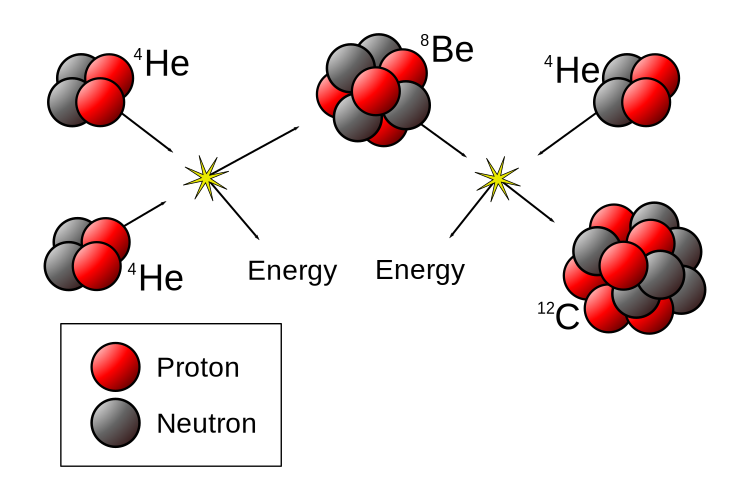
\includegraphics[width=0.5\textwidth]{../images/Triple-Alpha_Process.png}
\end{center}

The creation of 1 carbon nucleus from 3 helium nuclei releases $1.2\times 10^{-12}J$ of energy.

\begin{parts}
	\part[2] If the human body contains, on average, $1.6\times 10^{4}g$ of carbon and a carbon nucleus has a mass of $2\times 10^{-23}g$, about how many carbon atoms exist in the human body?
		\begin{TheSolution}
			We take the total mass of all the carbon atoms, divided by the mass/atom:
			\begin{eqnarray}
				\frac{1.6\times 10^4 g}{2\times 10^{-23} g/atom} = 0.8\times 10^{27} atoms = 8 \times 10^{26} atoms
			\end{eqnarray}
		\end{TheSolution}
	\part[2] If we assume all of this carbon was produced through the triple-alpha process in a star, then how many helium nuclei were consumed in the process?
		\begin{TheSolution}
			For every carbon atom produced, 3 helium nuclei were consumed:
			\begin{eqnarray}
			8 \times 10^{26} carbon \times \frac{3 helium}{1 carbon} = 24 \times 10^{26} helium = 2.4\times 10^{27} helium
			\end{eqnarray}
		\end{TheSolution}
	\part[2] How much energy was released to form the carbon contained in 1 average human?
		\begin{TheSolution}
			For every carbon atom produced, $1.2\times 10^{-12} J$ of energy was released.
			\begin{eqnarray}
			2.4\times 10^{27} nuclei \times \frac{1.2\times 10^{-12} J}{1 nucleus} = 2.88 \times 10^{15} J
			\end{eqnarray}
		\end{TheSolution}
\end{parts}

\clearpage
\bonusquestion[4] Science is a process people engage in, founded in the idea that through rigorous experimental testing we can refine our models of the world and thus better understand it. However, people are imperfect. What are some problems that arise when people engage in science?
\begin{TheSolution}
	There are a great many possible answers to this question. Some of the ones we covered in the first class include:
\begin{itemize}
	\item People have a tendency to double down on their opinions, rather than change them, when faced with contradicting evidence
\item People have biases and perspectives that prevent objectivity
\item People want the glory of a new discovery, therefore little effort is put into verifying experimental results.
\item ``Science" is seen as pure and objective, and associated with hard reasoning. It is therefore difficult to challenge an ``expert scientist" who can wield their titled when questioned (about motives, intention), conferring a position of authority
\item Science funding often dictates science project.
\end{itemize}
\end{TheSolution}

\end{questions}


\end{document}